\documentclass{article}
\usepackage{fullpage}
\title{KDETrees Simulations}
\author{Grady Weyenberg}
\usepackage{Sweave}
\begin{document}
\maketitle

\section{Introduction}
\label{sec:introduction}
Here we present the code for the simulations found in the KDETrees
article. These simulations compare the ability of KDETrees to find
trees which were generated by a non-contained coalescent process, in a
dataset consisting mostly of trees generated by a contained coalescent
process. We test two scenarios: all contained coalescent trees are
contained in a single species tree; and the contained coalescent trees
are sampled from a mixed distribution, where the trees are contained
in one of 5 different species trees. We also compare the performance
of our method with that of the previously published Phylo-MCOA method.

The coalescent trees are generated using the methods found in the
Dendropy python module. The script which generates the trees, as well
as the species trees can be found in the {\tt sim} directory of the
KDETrees package.

\section{Comparison of KDETrees and Phylo-MCOA}
\label{sec:comp-kdetr-phylo}
In this simulation we generate a test dataset which consists of one
``outlier'' tree, which is generated by an unconstrained coalescent
process, and 100 ``non-outlier'' trees which are generated by
constrained coalescent processes. The outlier trees used are those in
the {\tt species1.nex} file.
\begin{Schunk}
\begin{Sinput}
> out.trees <- read.nexus("sim/species1k.nex")
\end{Sinput}
\end{Schunk}
The non-outlier trees are created by the {\tt tresim.py} script.
This example call to the script will generate 100 coalescent trees
with effective population size 800 for each species tree found in
{\tt species.nex}.
\begin{Schunk}
\begin{Sinput}
> system2("sim/treesim.py",c("-s","sim/species.nex","-n",800,"-N",100))
\end{Sinput}
\end{Schunk}

Thus, each simulated dataset consists of a single tree from {\tt
  species1k.nex}, along with the output of a call to {\tt tresim.py}.

The simulation routine does the following for each outlier tree: (1)
generate the non-outlier trees, (2) call {\tt kdetrees}, in both
dissimilarity and topological modes, (3) call {\tt pMCOA} in both
modes, (4) determines whether or not the outlier tree is identified.
\begin{Schunk}
\begin{Sinput}
> sim <- function(neff,out.trees,sp.file="species.nex",ncoal=100,...){
+   found.kde <- integer(2)
+   found.pmcoa <- integer(2)
+   for (tree in .uncompressTipLabel(out.trees)){
+     trees <- read.tree(text=system2("sim/treesim.py",
+                          c("-n",neff,"-s",sp.file,"-N",ncoal),stdout=TRUE))
+     res.topo <- kdetrees(c(c(tree),trees),...,use.blen=FALSE)
+     res.diss <- kdetrees(c(c(tree),trees),...,use.blen=TRUE)
+     found.kde <- found.kde + c((1 %in% res.topo$outliers), (1 %in% res.diss$outliers))
+     
+     res.topo <- detect.complete.outliers(pMCOA(c(c(tree),trees),distance="nodal"))
+     res.diss <- detect.complete.outliers(pMCOA(c(c(tree),trees),distance="patristic"))
+     found.pmcoa <- found.pmcoa + c(res.topo$TFgn[1], res.diss$TFgn[1])
+   }
+   res <- c(found.kde,found.pmcoa)/length(out.trees) 
+   names(res) <- c("kde.topo","kde.diss","pmcoa.topo","pmcoa.diss")
+   res
+ }
\end{Sinput}
\end{Schunk}
The following wrapper runs the simulation for various effective
population sizes using {\tt mclapply}.
\begin{Schunk}
\begin{Sinput}
> sim2 <- function(out.trees,neff,nout=5,sp.file,ncoal=100){
+   result <- mclapply(neff,sim,out.trees,sp.file,ncoal,nout,mc.cores=4L)
+   out <- stack(as.data.frame(t(simplify2array(result))))
+   out$neff <- rep(neff,4)
+   out
+ }
\end{Sinput}
\end{Schunk}
Instead of the publised pMCOA routines, we use a slightly modified
version which removes most of the progress reporting present in the
published script.
\begin{Schunk}
\begin{Sinput}
> source("sim/my-pmcoa.R")
\end{Sinput}
\end{Schunk}

We run the simulation at 10 equally log-spaced values of the effective
population size.
\begin{Schunk}
\begin{Sinput}
> neff <- round(exp(seq(log(500),log(3000),len=10)))
\end{Sinput}
\end{Schunk}
This runs 100 simulation replicates with the contained coalescent
trees all generated using the single species tree shown in Figure \ref{fig:single-species}.
\begin{Schunk}
\begin{Sinput}
> result <- sim2(out.trees[1:100],neff,sp.file="sim/species.nex",ncoal=100)
\end{Sinput}
\end{Schunk}

\begin{figure}
  \centering
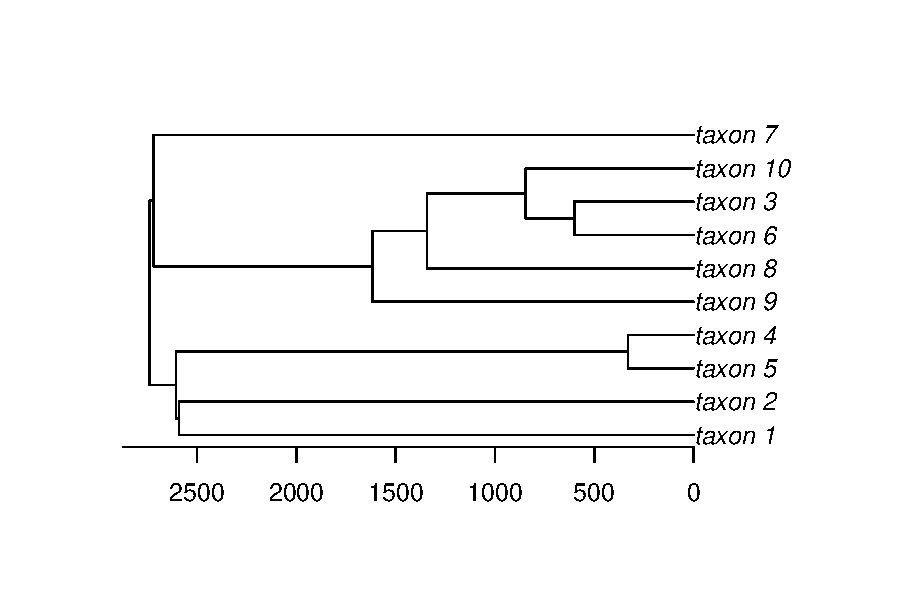
\includegraphics{simulation-008}
\caption{Species tree used for the single contained coalescent distribution simulation.}
  \label{fig:single-species}
\end{figure}

\begin{figure}
  \centering

\includegraphics{simulation-009}
  \caption{Species trees used for mixed coalescent simulation.}
\label{fig:mixed-species}  
\end{figure}

This run uses 5 species trees (see Figure \ref{fig:mixed-species}) to
generate the contained coalescent trees.
\begin{Schunk}
\begin{Sinput}
> mix.result <- sim2(out.trees[1:100],neff,sp.file="species5.nex",ncoal=20)
\end{Sinput}
\end{Schunk}
Format the results as a data frame suitable for use with
ggplot2. Results are shown in Figure \ref{fig:comparison}.
\begin{Schunk}
\begin{Sinput}
> sim1.res <- rbind(cbind(result,model="single"),cbind(mix.result,model="mixed"))
> sim1.res$Distance <- sim1.res$Method <- sim1.res$ind
> levels(sim1.res$Method) <- list(kdetrees=c("kde.outliers","kde.topo"),
+                                 pMCOA=c("pmcoa.outliers","pmcoa.topo"))
> levels(sim1.res$Distance) <- list(topographical=c("pmcoa.topo","kde.topo"),
+                                   dissimilarity=c("pmcoa.outliers","kde.outliers"))
\end{Sinput}
\end{Schunk}
\begin{figure}
  \centering
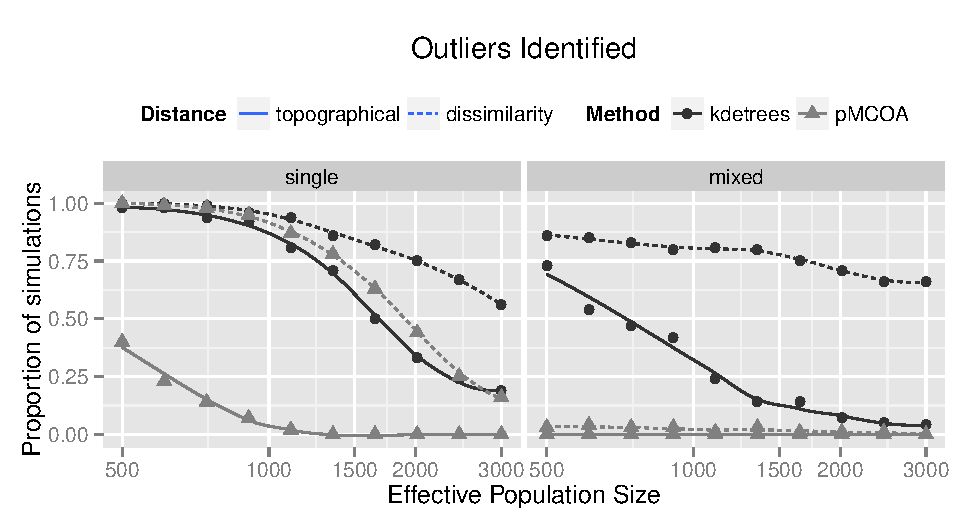
\includegraphics{simulation-013}
  \caption{Results of simulation comparing KDETrees with
    Phylo-MCOA. We find that in this situation, the branch-length
    methods outperform the topology-only methods for both KDETrees and
  Phylo-MCOA. More striking however is the complete failure of
  Phlyo-MCOA in the mixed distribution scenario, while KDETrees still
  performs quite well.}
  \label{fig:comparison}
\end{figure}

\section{Distribution of Tree Scores}
\label{sec:distr-tree-scor}
Also of interest to us is the distribution of tree scores, depending
on if the tree in question is an outlier tree or one of the contained
coalescent trees. If these score distributions have significant
overlap, then it will be difficult for the method to distinguish
between the two categories of trees. On the other hand, if the
distributions have little to no overlap, then identification of
outliers will be easier.

To do this, we generate 500 coalescent trees contained in the tree in
Figure \ref{fig:single-species}, and run kdetrees on these trees
alone to find the distribution of the non-outlier contained coalescent
trees. To find the distribution of outlier tree scores, one
non-contained tree from {\tt species1k.nex} is appended to the
contained trees, and the analysis re-run. This process is repeated for
many outlier trees, and their scores are recorded. Results of the
simulation are summarized in Figure \ref{fig:distributions}.
\begin{Schunk}
\begin{Sinput}
> simtrees <- read.tree(text=system2("./treesim.py",
+                         c("-n",1500,"-s","species.nex","-N",500),stdout=TRUE))
> sim2.res <- kdetrees(simtrees,use.blen=TRUE)
> dsim <- function(tree) kdetrees(c(c(tree),simtrees),use.blen=TRUE)$density[1]
> sim2.resa <- simplify2array(mclapply(out.trees[1:100],dsim,mc.cores=4L))
> sim2 <- rbind(cbind(data.frame(value=unname(sim2.res$density)),type="coalescent"),
+               cbind(data.frame(value=unname(sim2.resa)),type="outlier"))
\end{Sinput}
\end{Schunk}

\begin{figure}
  \centering
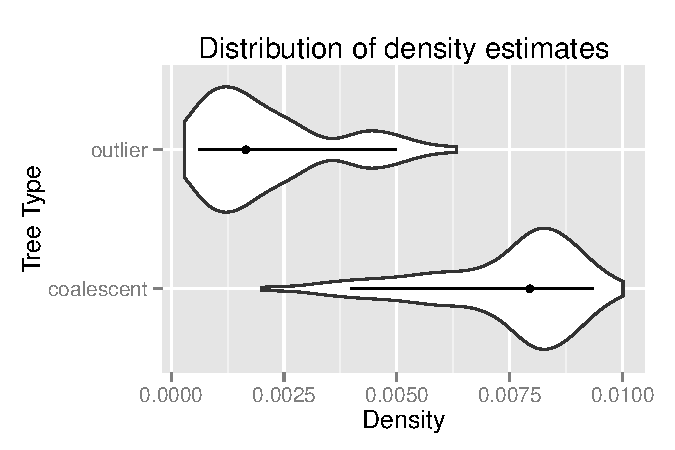
\includegraphics{simulation-015}
  \caption{Comparison of the distribution of density scores for outlier trees and the contained coalescent trees.}
  \label{fig:distributions}
\end{figure}

\end{document}
